\chapter{Unraveling the sequence determinants of environment-induced changes in pancreatic beta-cell states}
\label{chap:chapter 3}

%%%%%%%%%%%%%%%%%%%%%%%%%%%%%%%%%%%%%%%%%%%%%%%%%%%%%%%%%%%%%%%%%%%%%%%%%%%%%%%%
\section{Abstract}
%%%%%%%%%%%%%%%%%%%%%%%%%%%%%%%%%%%%%%%%%%%%%%%%%%%%%%%%%%%%%%%%%%%%%%%%%%%%%%%%

Pancreatic beta cell function is shaped by diverse environmental signals, many of which are relevant to the development of diabetes. However, the mechanisms by which these signals interact with genetic variation to influence gene regulation in beta cells remains incompletely understood. Here, we present a framework for identifying sequence determinants of environment-induced regulatory changes in beta-cell states. Using stem cell derived organoid model of human islets (SC-islets) exposed to four environmental stimuli across four timepoints, we profiled over 170k nuclei for paired gene expression and chromatin accessibility, and over 14k nuclei for paired DNA methylation and chromatin organization in SC-islets. We characterized condition-specific responses within each modality, identifying thousands of differentially expressed genes and accessible regions, particularly in response to inflammatory cytokines, and global methylation changes across conditions. We then trained sequence-to-function models to predict chromatin accessibility and CpG methylation from DNA sequence. Chromatin accessibility models captured cell type and condition-specific regulatory logic and showed strong performance in our evaluations of noncoding variant effect prediction. Our results support the use of multiomics in stimulated SC-islets as a framework to study context-dependent gene regulation and interpret genetic variants relevant to disease.

%%%%%%%%%%%%%%%%%%%%%%%%%%%%%%%%%%%%%%%%%%%%%%%%%%%%%%%%%%%%%%%%%%%%%%%%%%%%%%%%
\section{Main}
%%%%%%%%%%%%%%%%%%%%%%%%%%%%%%%%%%%%%%%%%%%%%%%%%%%%%%%%%%%%%%%%%%%%%%%%%%%%%%%%

Pancreatic islets are small clusters of endocrine cells that regulate the metabolism of glucose. Among the endocrine cell types, beta cells play a central role by producing and secreting insulin in response to intrinsic and extrinsic signals \cite{Prentki2013-vx}. While glucose is the principal stimulus for beta cell mediated insulin secretion, beta cell function is also modulated by an array of additional signals, including fatty acids \cite{Fu2013-cf,Mauvais-Jarvis2016-gm,Ramos-Rodriguez2019-ha,Aylward2021-nw}, amino acids (\textit{citation needed}), incretin hormones \cite{Saxena2010-ui}, proinflammatory cytokines \cite{Benaglio2022-rq}, glucocorticoids \cite{Aylward2021-nw,Reddy2009-qu}, and sex hormones \cite{Mauvais-Jarvis2016-gm}. A few of these environmental cues have been shown to alter the broader transcriptional and epigenomic landscape of beta cells \cite{Aylward2021-nw,Benaglio2022-rq,Ramos-Rodriguez2019-ha}, revealing widespread, time-dependent changes in histone modifications, chromatin accessibility, and gene expression \cite{Ramos-Rodriguez2019-ha,Benaglio2022-rq}. These responses primarily reflect modulation of pre-existing cis-regulatory elements (CREs), which are frequently enriched for both transcription factor (TF) binding motifs relevant to the applied stimulus and glucose-associated genetic variants identified through genome-wide association studies.

% Variants identified through genome-wide association studies (GWAS) of metabolic traits and related diseases, such as fasting glucose \cite{Ingelsson2010-tw,Manning2012-ro,Scott2012-hq,Wood2017-uc,Williamson2023-gf} and type 2 diabetes \cite{Dupuis2010-ws,Morris2012-uu,Mahajan2022-hu} respectively, are strongly enriched in CREs active in pancreatic islets \cite{Liu2016-on,Pasquali2014-cu}. Within islets, this enrichment is pronounced in regulatory regions specific to beta cells \cite{Chiou2021-ro}. For instance, variants near MTNR1B, a locus contributing substantially to fasting glucose heritability, have been shown to alter beta cell enhancer activity \cite{Prokopenko2009-ou}. More comprehensively elucidating the mechanisms by which noncoding variants impact beta-cell regulatory programs remains a major challenge, particularly when a certain environmental context is necessary for the effect to be observed.

Given the central role of islets in diabetes pathogenesis, the islet epigenome has been the focus of extensive investigation \cite{Pasquali2014-cu,Gaulton2010-mq,Greenwald2019-ou,Khetan2018-fm,Thurner2018-ln,Volkov2017-tz}. Most of these data have been derived from bulk islet tissue, limiting the ability to resolve contributions from individual cell types. Recent advances in single-cell technologies have enabled high-resolution epigenomic profiling at the level of individual cells. Including multimodal platforms that simultaneously measure combinations of chromatin accessibility, gene expression, DNA methylation, and three-dimensional genome architecture \cite{Lee2019-qo,Liu2021-km}. Our group and others have recently generated single-cell chromatin accessibility maps from healthy human islets, revealing regulatory elements active in beta cells and uncovering previously unappreciated heterogeneity within the beta-cell population \cite{Chiou2021-ro,Rai2020-cf,Wang2023-me}.

However, primary human islets are not amenable to genetic manipulation, which limits their utility for validating the functional consequences of these variants. Transformed human beta cell lines \cite{Ravassard2011-lj} offer an alternative but face significant limitations, including poor single-cell growth and the absence of interactions with other endocrine cell types \cite{Rutter2013-yv}. Human pluripotent stem cell (hPSC)-derived islet organoids (SC-islets) help overcome these barriers by recapitulating the major endocrine populations present in native islets \cite{Hogrebe2020-rr,Rezania2014-nz,Veres2019-qb,Velazco-Cruz2019-yq,Zhu2023-qm} while providing a genetically tractable system for targeted genome editing. CRISPR-based perturbations in hPSC-islet organoids have enabled both fine-scale dissection of individual regulatory elements and scalable functional screening.

Deep learning models trained directly on genomic sequence have shown strong performance in predicting a range of regulatory phenotypes \cite{Sasse2024-ly}. These sequence-to-function models learn sequence features, including TF binding site syntax and combinatorial motif logic, that are predictive of chromatin accessibility \cite{Pampari2025-lm}, gene expression\cite{Linder2025-or}, DNA methylation\cite{Zeng2017-kb}, and three-dimensional chromatin conformation \cite{Fudenberg2020-gs}. Because they operate on sequence alone, these models provide a natural framework for evaluating functional consequences of noncoding variants by comparing predicted outputs for reference and alternate alleles. Recently, they’ve seen success in prioritization of variants affecting chromatin accessibility in Type 2 diabetes \cite{Hudaiberdiev2023-ew}. As such, they represent a valuable tool for decoding the regulatory genome and prioritizing candidate variants associated with disease-relevant traits. 

\subsection{Multiomic profiling of stem-cell derived pancreatic organoids}

\begin{figure}[p]
    \centering
    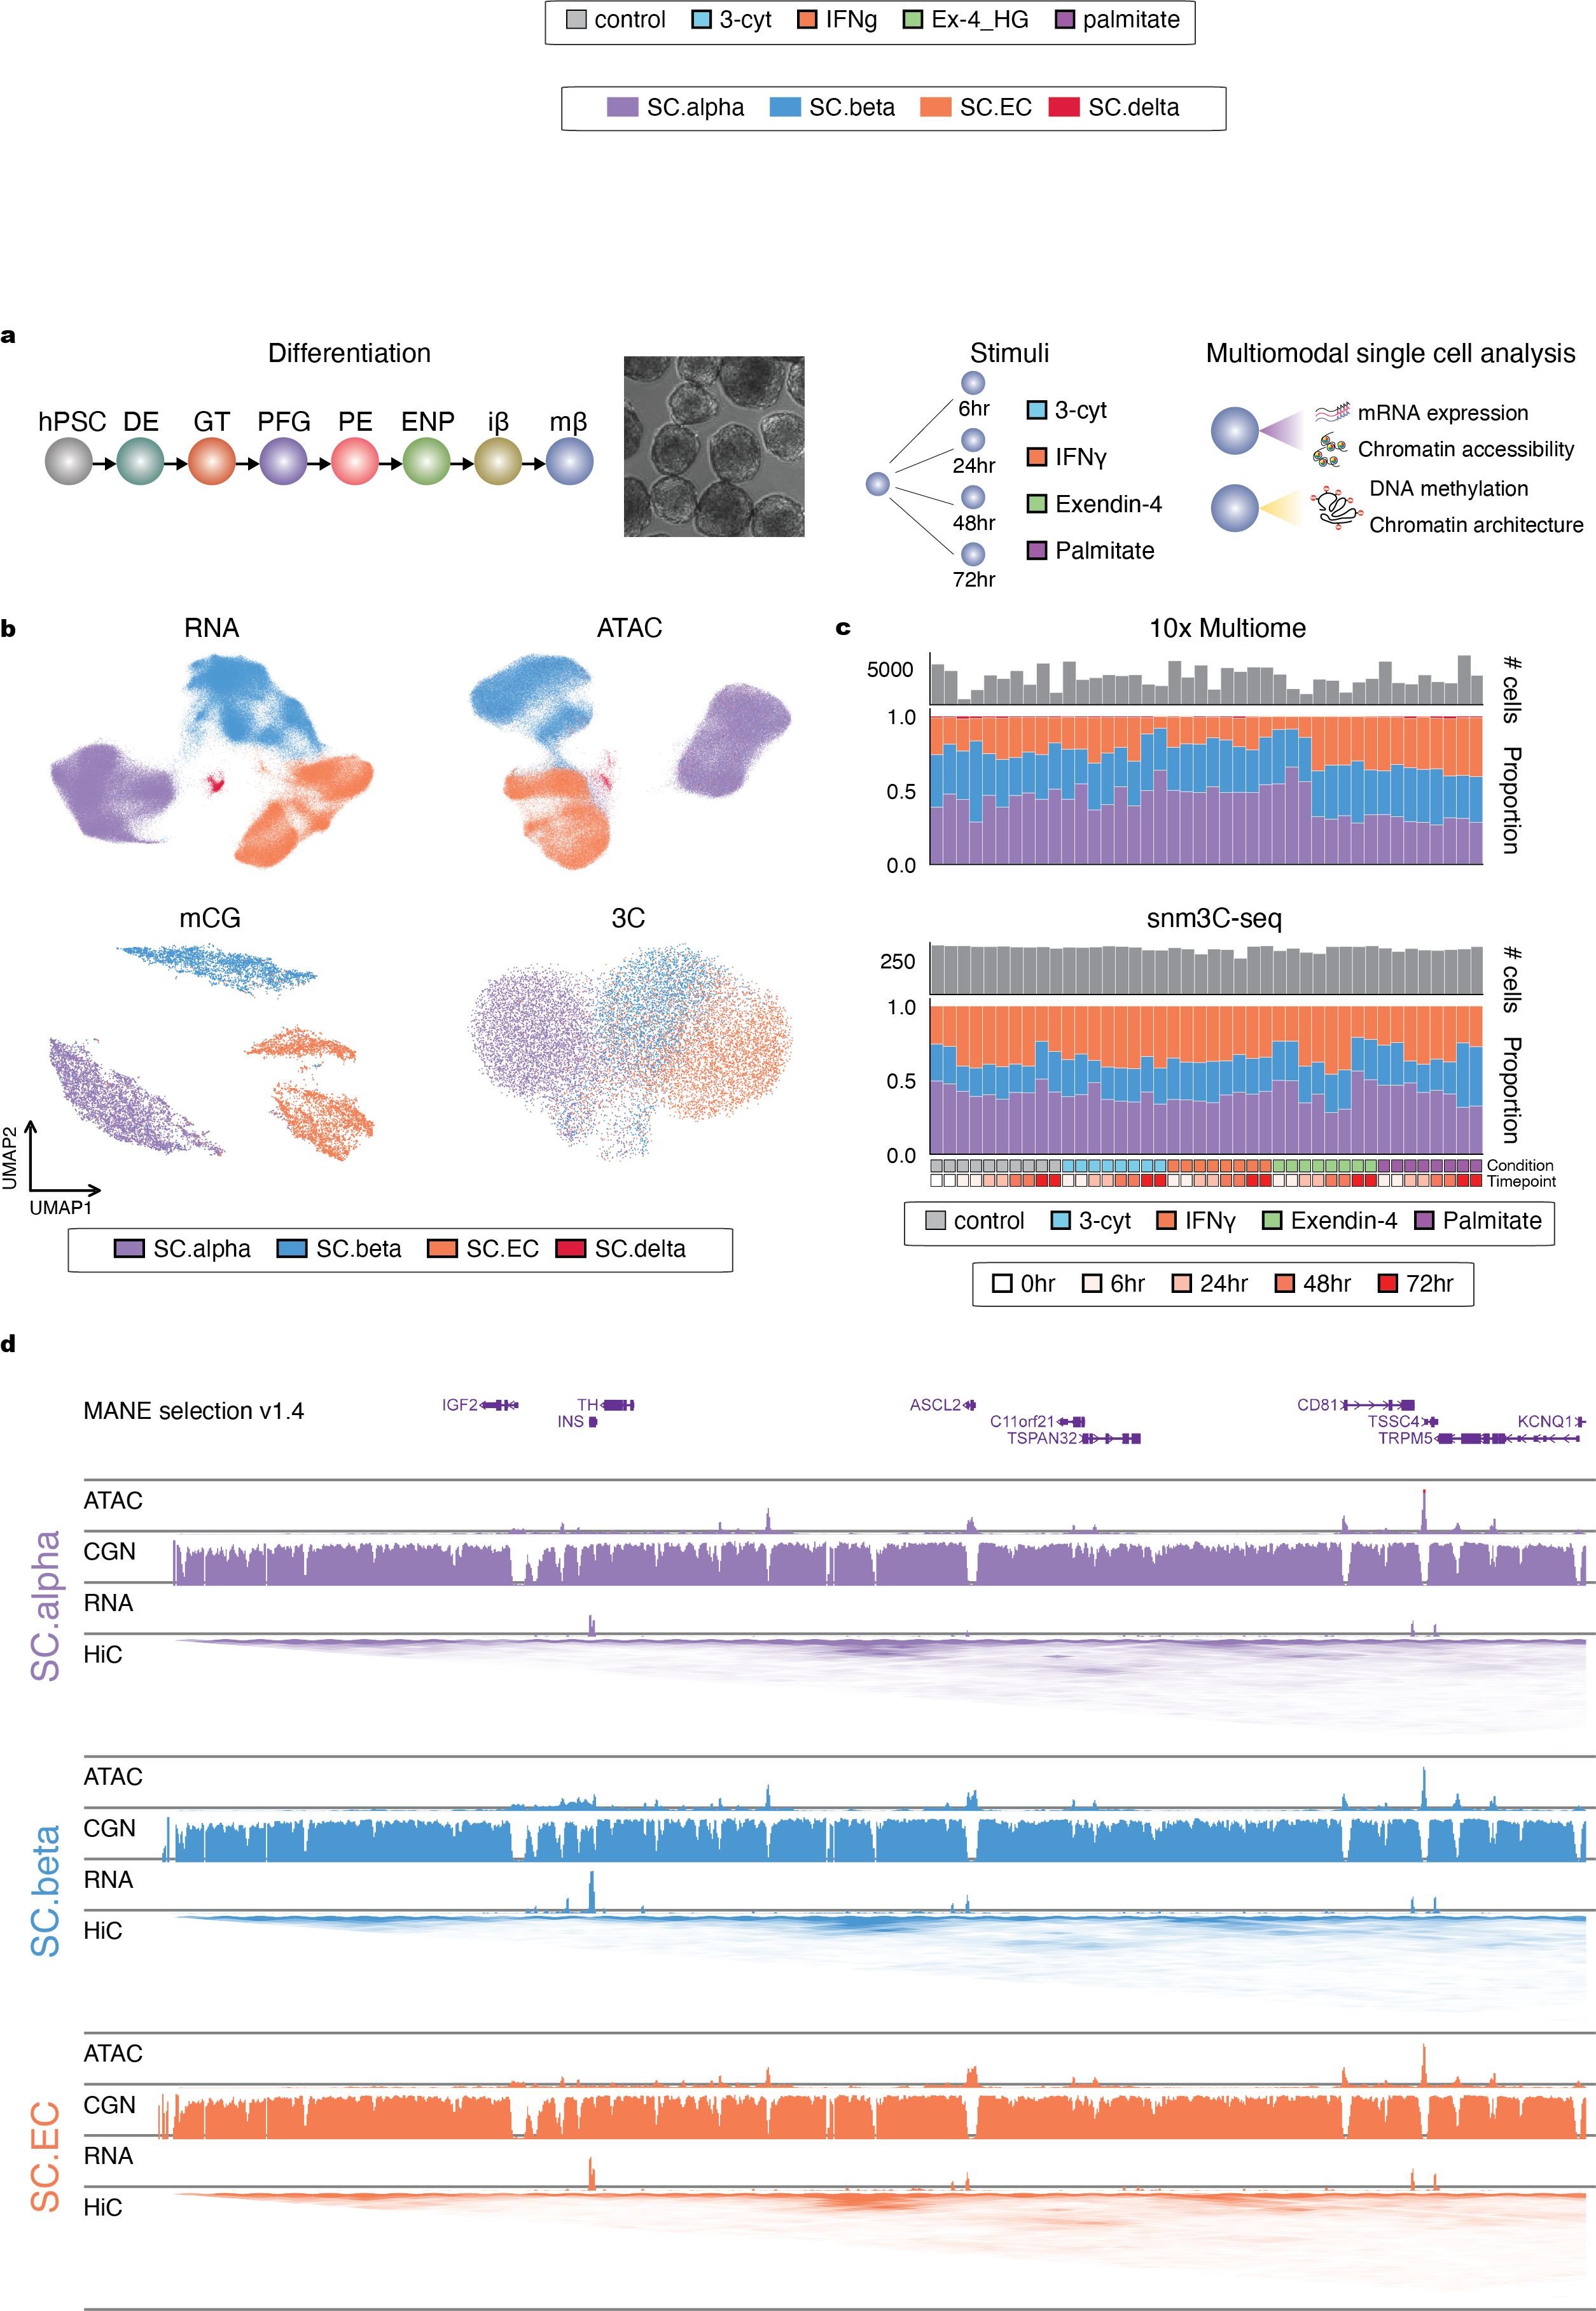
\includegraphics[width=0.9\textwidth, height=0.745\textheight]{3_figures-and-files/Fig1.png}
    \caption[Multiomic profiling of hPSC-derived islet organoids]{\textbf{Multiomic profiling of hPSC-derived islet organoids across environmental conditions}. \textbf{a}, Schematic of directed differentiation from H1 hPSCs into islet organoids followed by stimulation with one of four environmental conditions across four time points. Multiomic single-cell assays were used to capture single-cell mRNA, chromatin accessibility, DNA methylation and chromatin conformation profiles. \textbf{b}, UMAP embeddings showing cell type labels divided by mRNA expression (RNA), chromatin accessibility (ATAC), DNA methylation (mCG), and 3D chromatin contacts (3C) across all conditions. \textbf{c}, Bar plots showing the number and relative proportion of cells per cell type across conditions and time points for 10x Multiome and snm3C-seq. \textbf{d}, Representative genome browser tracks at the INS locus and downstream showing chromatin accessibility, DNA methylation, mRNA expression and HiC profiles for SC-alpha, SC-beta, and SC-EC cells aggregated across all conditions.}
    \label{fig:3 Figure 1}
\end{figure}

To investigate the temporal response of $\beta$ cells to environmental signals, we first differentiated H1 human pluripotent stem cells (hPSCs) through a stepwise protocol into SC-islets (\textbf{Figure~\ref{fig:3 Figure 1}\textbf{a}}) \cite{Hogrebe2020-rr,Rezania2014-nz,Veres2019-qb,Velazco-Cruz2019-yq,Zhu2023-qm}. Following differentiation, we introduced four different stimuli to the cell culture media: 1) a cocktail of three cytokines (3-cyt), 2) IFN$\gamma$ alone (IFN$\gamma$), 3) Exendin-4 in the presence of high glucose (Exendin-4), and 4) palmitate. We collected aliquots of each treated culture at four time points (6, 24, 48, and 72 hours), alongside a control time course of unstimulated organoids with an additional baseline timepoint (0 hr). Two replicates were done for each timepoint-condition combination. We then performed multiomic single-cell profiling across conditions and timepoints using two assays. Using the 10x Genomics Multiome platform, we simultaneously measured chromatin accessibility and gene expression from the same nuclei. In parallel, we applied snm3C-seq to jointly profile DNA methylation and 3D chromatin architecture \cite{Liu2021-km}. Each sample was subjected to systematic quality control to filter out low quality nuclei (\textbf{Supplementary Figure~\ref{fig:3 supplementary_1}}, \textbf{Supplementary Table 1}, see Methods). In total, we profiled 171{,}815 nuclei using 10x Multiome and 14{,}197 nuclei using snm3C-seq.

We performed unsupervised clustering on gene expression (10x Multiome) and DNA methylation (snm3C-seq) profiles to identify major islet endocrine cell types (\textbf{Figure~\ref{fig:3 Figure 1}\textbf{c}}, \textbf{Supplementary Figure~\ref{fig:3 supplementary_1}\textbf{a}}). Cell type labels were assigned based on known marker genes (\textbf{Supplementary Figure~\ref{fig:3 supplementary_1}\textbf{b}}), with clusters corresponding to SC-$\alpha$ cells (purple), SC-$\beta$ (blue), SC-EC (orange), and SC-$\delta$ (red) cells. While SC-$\delta$ cells were readily identifiable in expression space (RNA) via \textit{SST} expression, they did not form distinct clusters in the DNA methylation space, likely reflecting their low abundance or less distinctive methylation profile in this context. We examined cell type proportions across stimuli and time points for each assay (\textbf{Figure~\ref{fig:3 Figure 1}\textbf{e}}). Despite differences in the number of cells captured per condition, the relative distribution of SC-$\alpha$, SC-$\beta$, and SC-EC cells remained broadly consistent across assays and conditions. To facilitate downstream comparisons between molecular modalities, we aggregated sequencing reads within each cell type to construct cell type resolved transcriptome and epigenome maps at multiple resolutions, including across all measured conditions (\textbf{Figure~\ref{fig:3 Figure 1}\textbf{h}}). At a sample level, pseudobulked modalities exhibited strong correlation in the expected directions across genes (\textbf{Supplementary Figure~\ref{fig:3 supplementary_2}\textbf{c}}).

\subsection{Treatments induce variable transcriptomic response in SC-beta cells}

\begin{figure}[p]
    \centering
    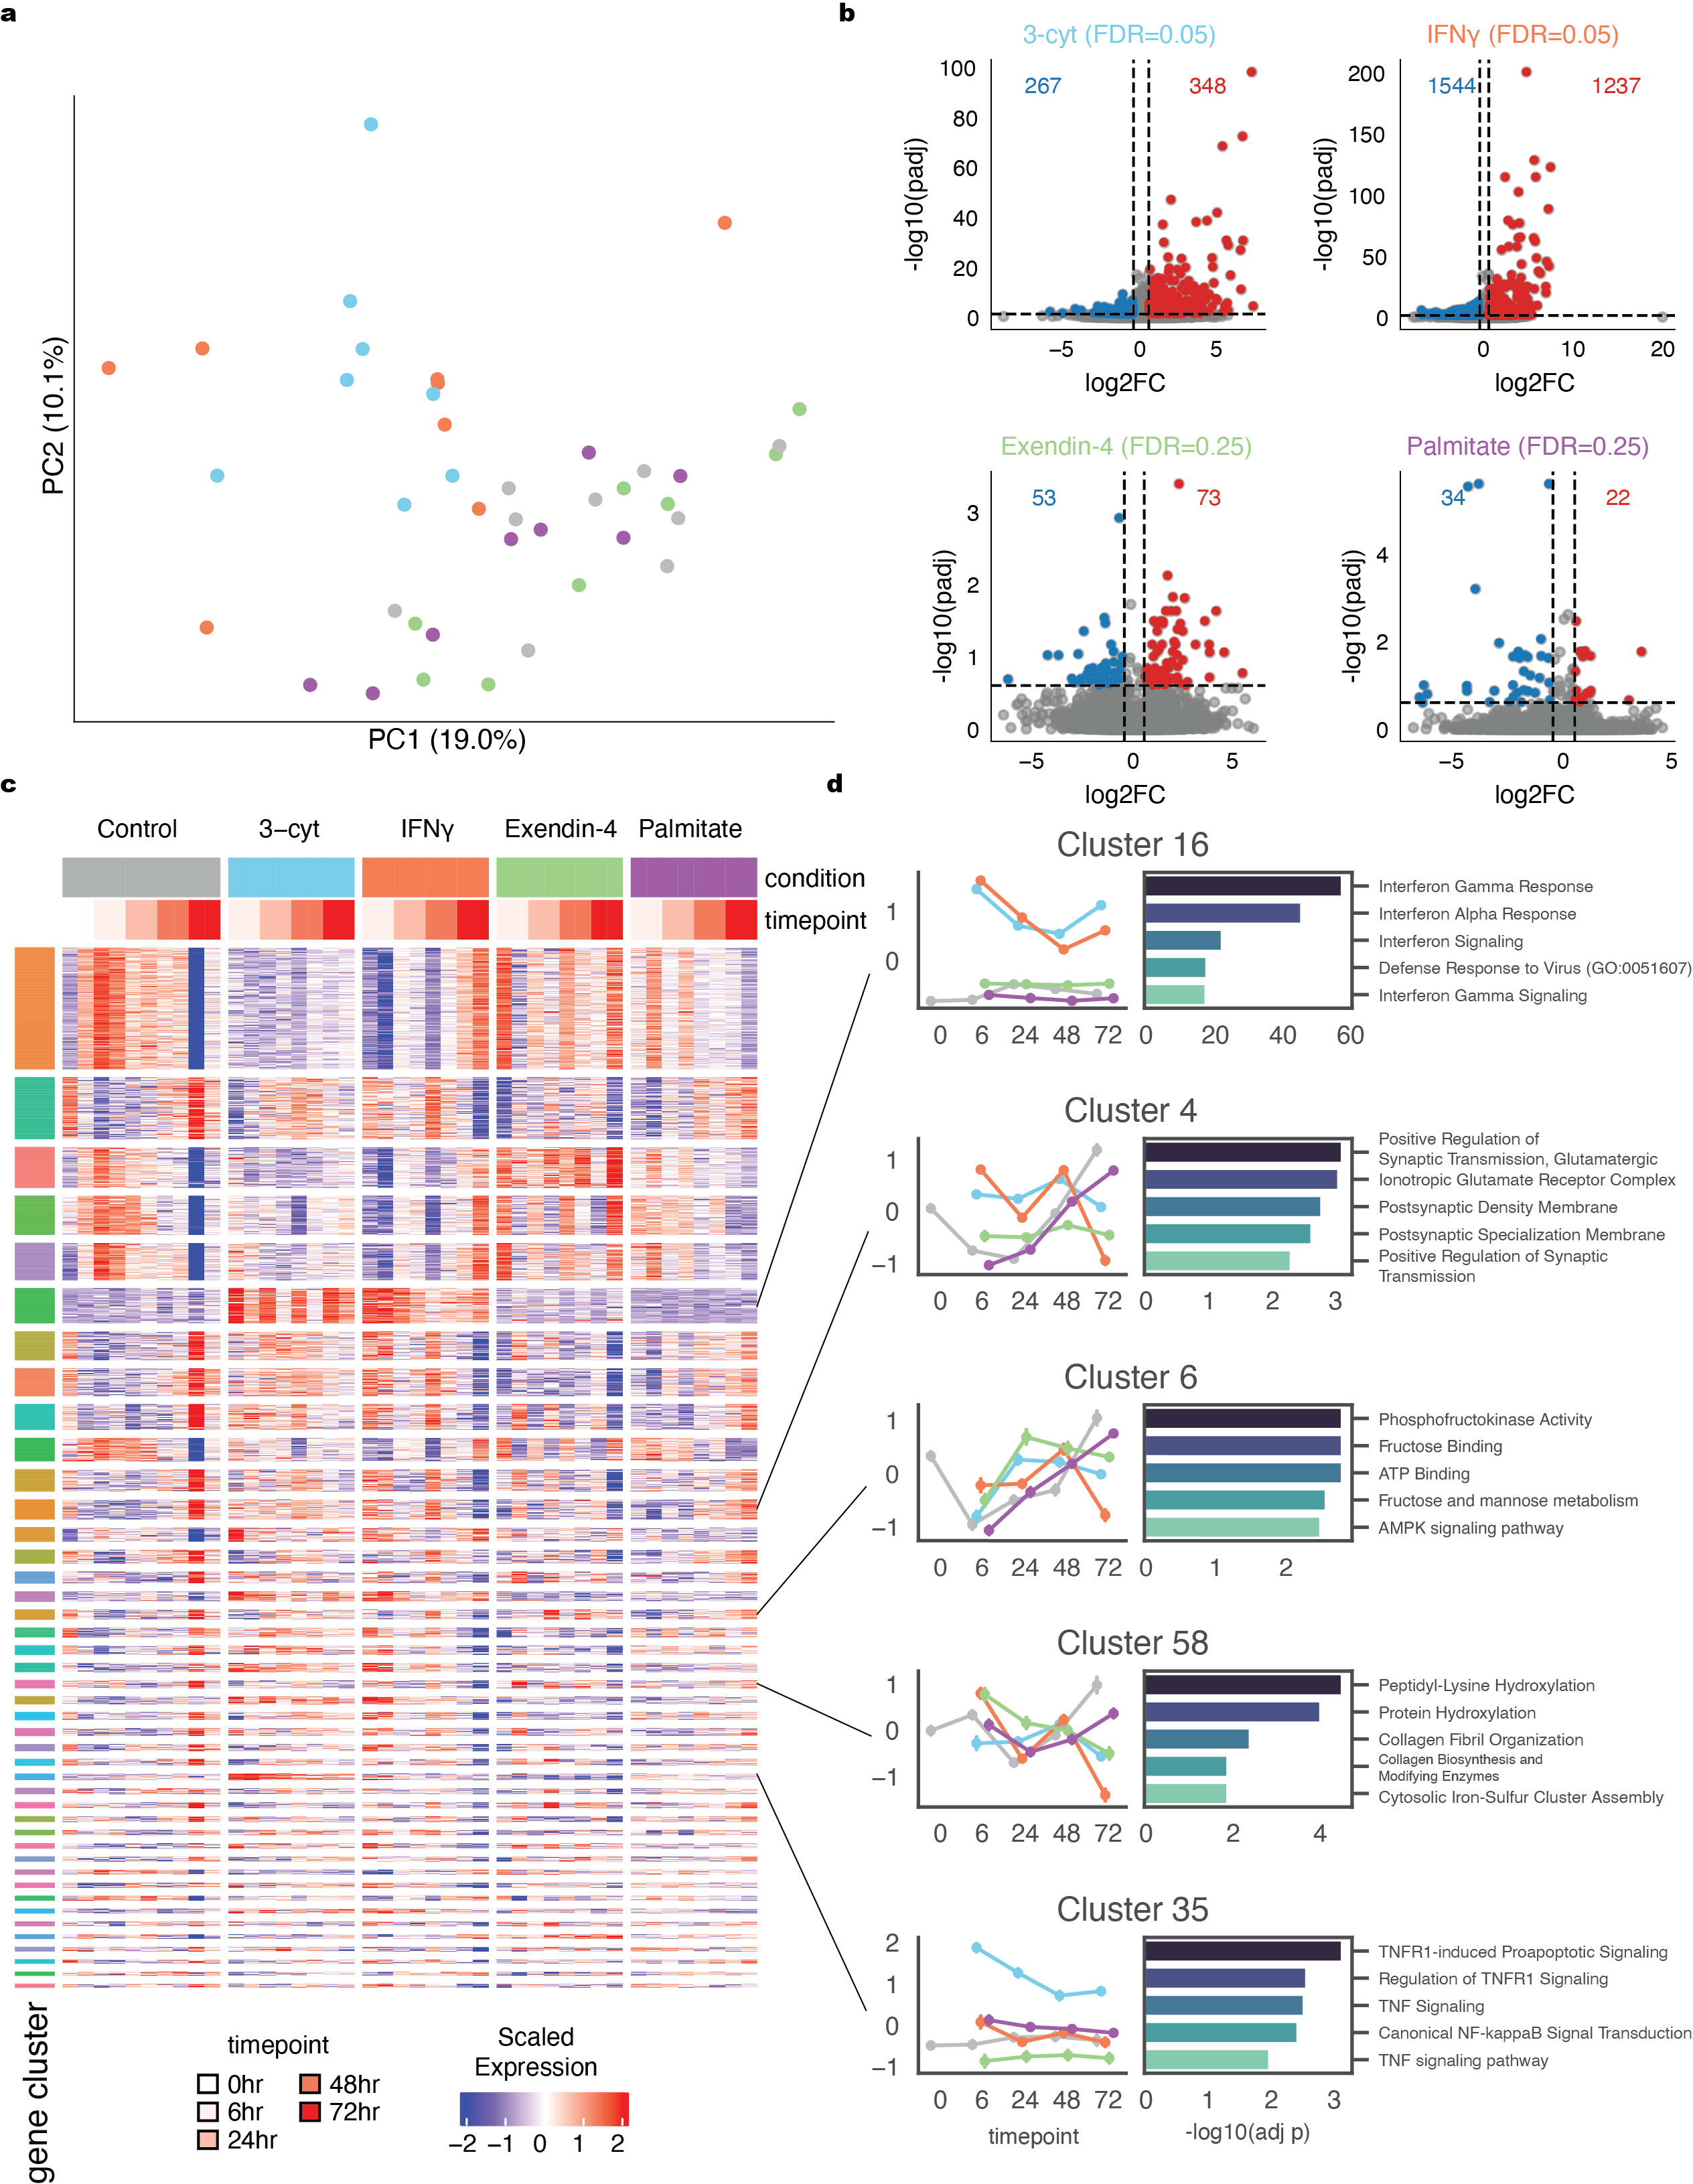
\includegraphics[width=0.9\textwidth, height=0.745\textheight]{3_figures-and-files/Fig2.png}
    \caption[Transcriptomic responses of SC-beta cells]{\textbf{Transcriptomic responses of SC-beta cells to environmental stimuli}. \textbf{a}, Principal component analysis of pseudobulked SC-beta cell transcriptomes across all conditions and time points. Each point represents a sample, colored by treatment. \textbf{b}, Volcano plots showing differentially expressed genes in SC-beta cells at any time point relative to control for each stimulus. From top left to bottom right: 3-cyt, IFNg, exendin-4, and palmitate. Red points denote genes with log2FC > 0.5 and FDR < threshold (0.05 for cytokines, 0.25 for exendin-4, and palmitate). Blue points denote genes with log2FC < 0.5 and FDR < threshold. Numbers indicate up- and down-regulated genes. \textbf{c}, Heatmap of Z-scored gene expression across time points for each treatment in SC-beta cells. DEGs are grouped into clusters based on temporal expression dynamics. \textbf{d}, Representative expression profiles for five selected gene clusters across the time course. Right panels show GO term enrichments associated with each cluster (top five terms shown, ordered by adjusted p-value).}
    \label{fig:3 Figure 2}
\end{figure}

To assess how each stimulus affected gene expression in SC-$\beta$ cells, we first generated pseudobulk transcriptomes by aggregating snRNA-seq UMI counts across SC-$\beta$ labeled cells from each sample. We then performed differential gene expression analysis using DESeq2 to identify genes with condition-specific changes at any point across the time course (see Methods). We observed the strongest transcriptomic responses in SC-$\beta$ cells exposed to proinflammatory cytokines (\textbf{Figure~\ref{fig:3 Figure 2}\textbf{a}}), with 3-cyt and IFN$\gamma$ inducing 615 and 2,781 differentially expressed genes (DEGs) respectively at an FDR of 5\% (\textbf{Figure~\ref{fig:3 Figure 2}\textbf{b}}). In contrast, Exendin-4 and palmitate induced subtler changes (\textbf{Figure~\ref{fig:3 Figure 2}\textbf{b}}), with 126 and 46 DEGs respectively at an FDR of 25\%. Notably, several of the genes induced by Exendin-4, including \textit{SLC8A1} \cite{Hamming2010-td}, \textit{PDK4} \cite{Arumugam2010-bq}, and \textit{TXNIP}, are known components of the $\beta$-cell response to glucose stimulation. \textit{TXNIP}, in particular, has been reported to be strongly upregulated in diabetic islets and is linked to $\beta$-cell stress responses \cite{Rutter2013-yv}. A significant proportion of DEGs were shared among 3-cyt and IFN$\gamma$ responses and the Exendin-4 and IFN$\gamma$, but we observed minimal overlap among other conditions (\textbf{Supplementary Figure~\ref{fig:3 supplementary_3}\textbf{a}}).

Using decoupleR \cite{Badia-I-Mompel2022-se}, we inferred TF activities across conditions (\textbf{Supplementary Figure~\ref{fig:3 supplementary_3}\textbf{b}}). The cytokine treatments (3-cyt, IFN$\gamma$) prominently activated downstream targets of known immune regulators of $\beta$ cells including \textit{STAT1}, \textit{IRF1}, and \textit{CIITA} \cite{Benaglio2022-rq}. As expected, NF-$\kappa$B was upregulated in 3-cyt and not IFN$\gamma$ \cite{Melloul2008-ox}. Under palmitate treatment, we observed reduced activity of \textit{HNF1B} and \textit{ISL1}, both of which are essential for maintaining mature $\beta$-cell identity \cite{El-Khairi2016-so,Ediger2014-gk}. \textit{TFEB}, a regulator of lysosomal biogenesis and autophagy, was strongly upregulated in response to Exendin-4, consistent with reports that GLP-1 agonists activate \textit{TFEB} via calcium/calcineurin signaling to enhance autophagic flux and improve $\beta$ cell survival \cite{Zummo2022-dr}. In contrast, \textit{TFEB} activity was consistently suppressed in response to both palmitate and cytokines. Exendin-4 also led to downregulation of several \textit{GATA6} targets, consistent with studies showing that \textit{GATA6} knockdown impairs $\beta$ cell function and identity \cite{Villamayor2018-uk}. \textit{PIAS1} was one of the few transcriptional regulators significantly upregulated under Exendin-4 treatment. As an E3 SUMO ligase, \textit{PIAS1} modulates post-translational SUMOylation of TFs, a pathway previously implicated in $\beta$ cell stress adaptation and survival \cite{Li2020-kg}.

To further resolve shared and condition-specific transcriptional responses, we performed unsupervised clustering of differentially expressed genes across all conditions, identifying 43 gene clusters (\textbf{Figure~\ref{fig:3 Figure 2}\textbf{c}}). Gene ontology enrichment analysis revealed that these clusters capture a range of functional annotations (\textbf{Figure~\ref{fig:3 Figure 2}\textbf{d}}). For example, Cluster 16 genes exhibited an immediate and sustained upregulation in response to cytokine treatments and were strongly enriched for terms related to interferon signaling. Cluster 4 genes were induced at later time points in the palmitate and control conditions and were enriched for synaptic signaling and glutamate receptor activity. Cluster 6 genes were also marked by a delayed upregulation most pronounced under palmitate exposure and included genes involved in fructose metabolism and AMPK signaling. Cluster 58 genes included those involved in structural remodeling programs, with enrichment for collagen organization and hydroxylation pathways that increased at later time points in palmitate and control. As a final example, Cluster 35 captured canonical inflammatory stress responses to TNF$\alpha$ signaling and was sharply induced by only the 3-cytokine cocktail. These clusters highlight the range of early and delayed gene programs engaged across stimuli, spanning immune activation, metabolic compensation, and cell structure remodeling.

\subsection{Cytokines induce strong changes in chromatin accessibility}

\begin{figure}[p]
    \centering
    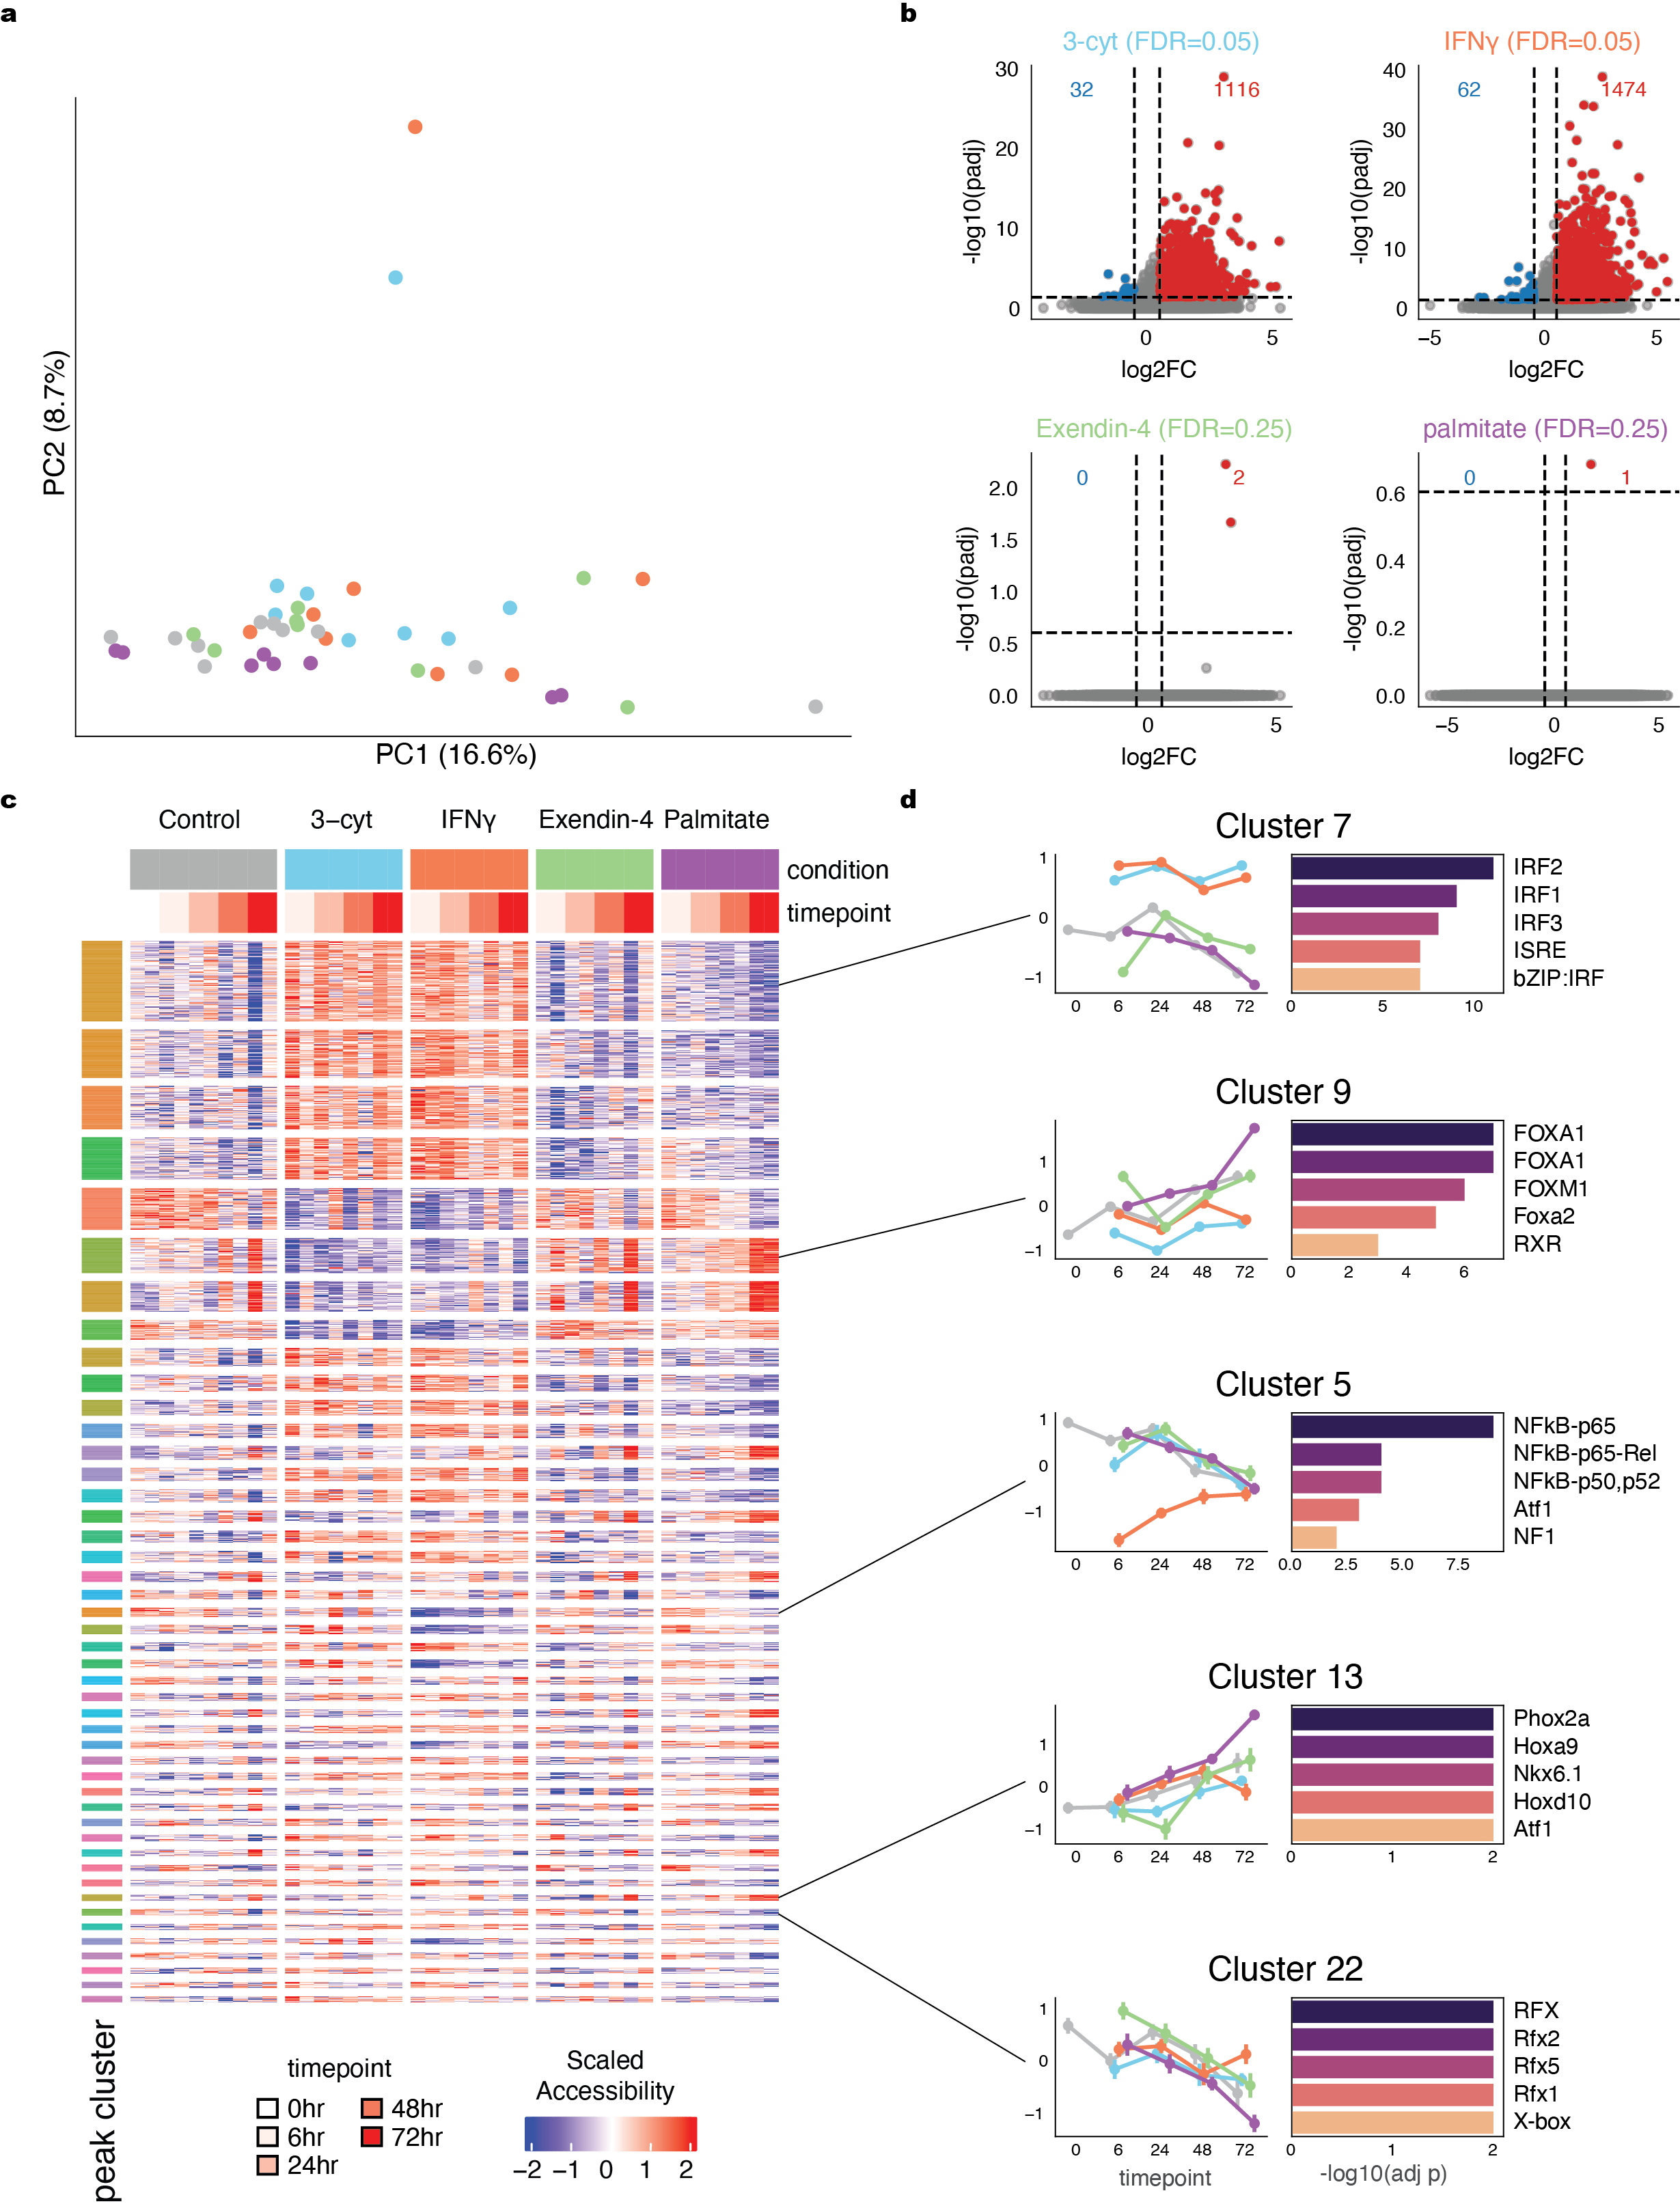
\includegraphics[width=0.9\textwidth, height=0.745\textheight]{3_figures-and-files/Fig3.png}
    \caption[Chromatin accessibility dynamics in SC-beta cells]{\textbf{Chromatin accessibility dynamics in SC-beta cells in response to environmental stimuli}. \textbf{a}, Principal component analysis of pseudobulk chromatin accessibility profiles from SC-beta cells across all conditions and time points. \textbf{b}, Volcano plots showing differentially accessible peaks in SC-beta cells at any time point relative to baseline for each stimulus. From top left to bottom right: 3-cyt, IFNg, exendin-4, and palmitate. Red points denote peaks with log2FC > 0.5 and FDR < threshold (0.05 for cytokines, 0.25 for exendin-4, and palmitate). Blue points denote peaks with log2FC < 0.5 and FDR < threshold. Numbers indicate up- and down-regulated genes. \textbf{c}, Heatmap showing Z-scored accessibility for dynamic peaks across time points and conditions in SC-beta cells. DARs are grouped into clusters based on temporal accessibility profiles. \textbf{d}, Representative accessibility profiles for five selected clusters, with HOMER motif enrichment results shown on the right. Top five enriched motifs per cluster are listed and ranked by adjusted p-value.}
    \label{fig:3 Figure 3}
\end{figure}

% We next performed a parallel analysis to evaluate how environmental stimuli influence chromatin accessibility in SC-$\beta$ cells. As with the transcriptomic analysis, we aggregated Tn5 insertion counts in our consensus peak set (see Methods) and performed differential accessibility analysis for each condition relative to baseline using DESeq2. The largest changes in SC-$\beta$ chromatin accessibility were again observed in response to cytokine exposure (\textbf{Figure~\ref{fig:3 Figure 3}\textbf{a}}). Treatment with 3-cyt and IFN$\gamma$ led to 1,148 or 1,536 differentially accessible peaks, respectively (\textbf{Figure~\ref{fig:3 Figure 3}\textbf{b}}). Almost all peaks increased in accessibility, with a large proportion of upregulated differentially accessible regions (DARs) shared among the cytokine treatments (\textbf{Supplementary Figure~\ref{fig:3 supplementary_3}\textbf{c}}). In contrast, Exendin-4 and palmitate induced negligible chromatin changes, even at a relaxed FDR threshold of 25\% (\textbf{Figure~\ref{fig:3 Figure 3}\textbf{b}}). We observed subtle but significant differences in peak annotation and distance from the TSS (\textbf{Supplementary Figure~\ref{fig:3 supplementary_3}\textbf{d}}) between differential and non-induced peaks. Overall, these results suggest that cytokines drive coordinated changes in both gene expression and cis-regulatory activity in SC-$\beta$ cells.

% We next clustered differentially accessible peaks across the time course, identifying 46 distinct patterns of accessibility dynamics (\textbf{Figure~\ref{fig:3 Figure 3}\textbf{c}}). TF motif enrichment analysis using HOMER \cite{Heinz2010-yo} uncovered clear regulatory signatures across clusters. Cytokine treatments produced the most pronounced chromatin changes, with multiple clusters showing sharp changes in accessibility. For example, Cluster 7 peaks showed strong induction in both the 3-cyt and IFN$\gamma$ conditions and were enriched for IRF and STAT motifs, consistent with interferon signaling. Cluster 5 peaks showed a rapid but IFN$\gamma$-specific decrease in accessibility, and were enriched for NF-$\kappa$B motifs. In contrast, palmitate induced more modest chromatin changes, but several peak clusters showed delayed stimulation unique to this condition. Cluster 9 and Cluster 23 peaks, for instance, exhibited a gradual increase in accessibility under palmitate and were enriched for FOX family motifs and an \textit{NKX6-1} motif respectively, both key regulators of $\beta$ cell identity and function \cite{Geusz2021-mr,Lantz2004-mi,Aigha2020-uu}. Cluster 22, on the other hand, exhibited a gradual decrease in accessibility and was enriched for RFX motifs \cite{Piccand2014-bd}. This suggests that palmitate gradually activates regulatory elements linked to FOXA and \textit{NKX6-1}, while repressing RFX-associated regions over time, a shift that may mark a transition from compensatory to dysfunctional $\beta$ cell states.

\subsection{Sequence-to-function neural networks capture chromatin accessibility and predict variant effects}

\begin{figure}[p]
    \centering
    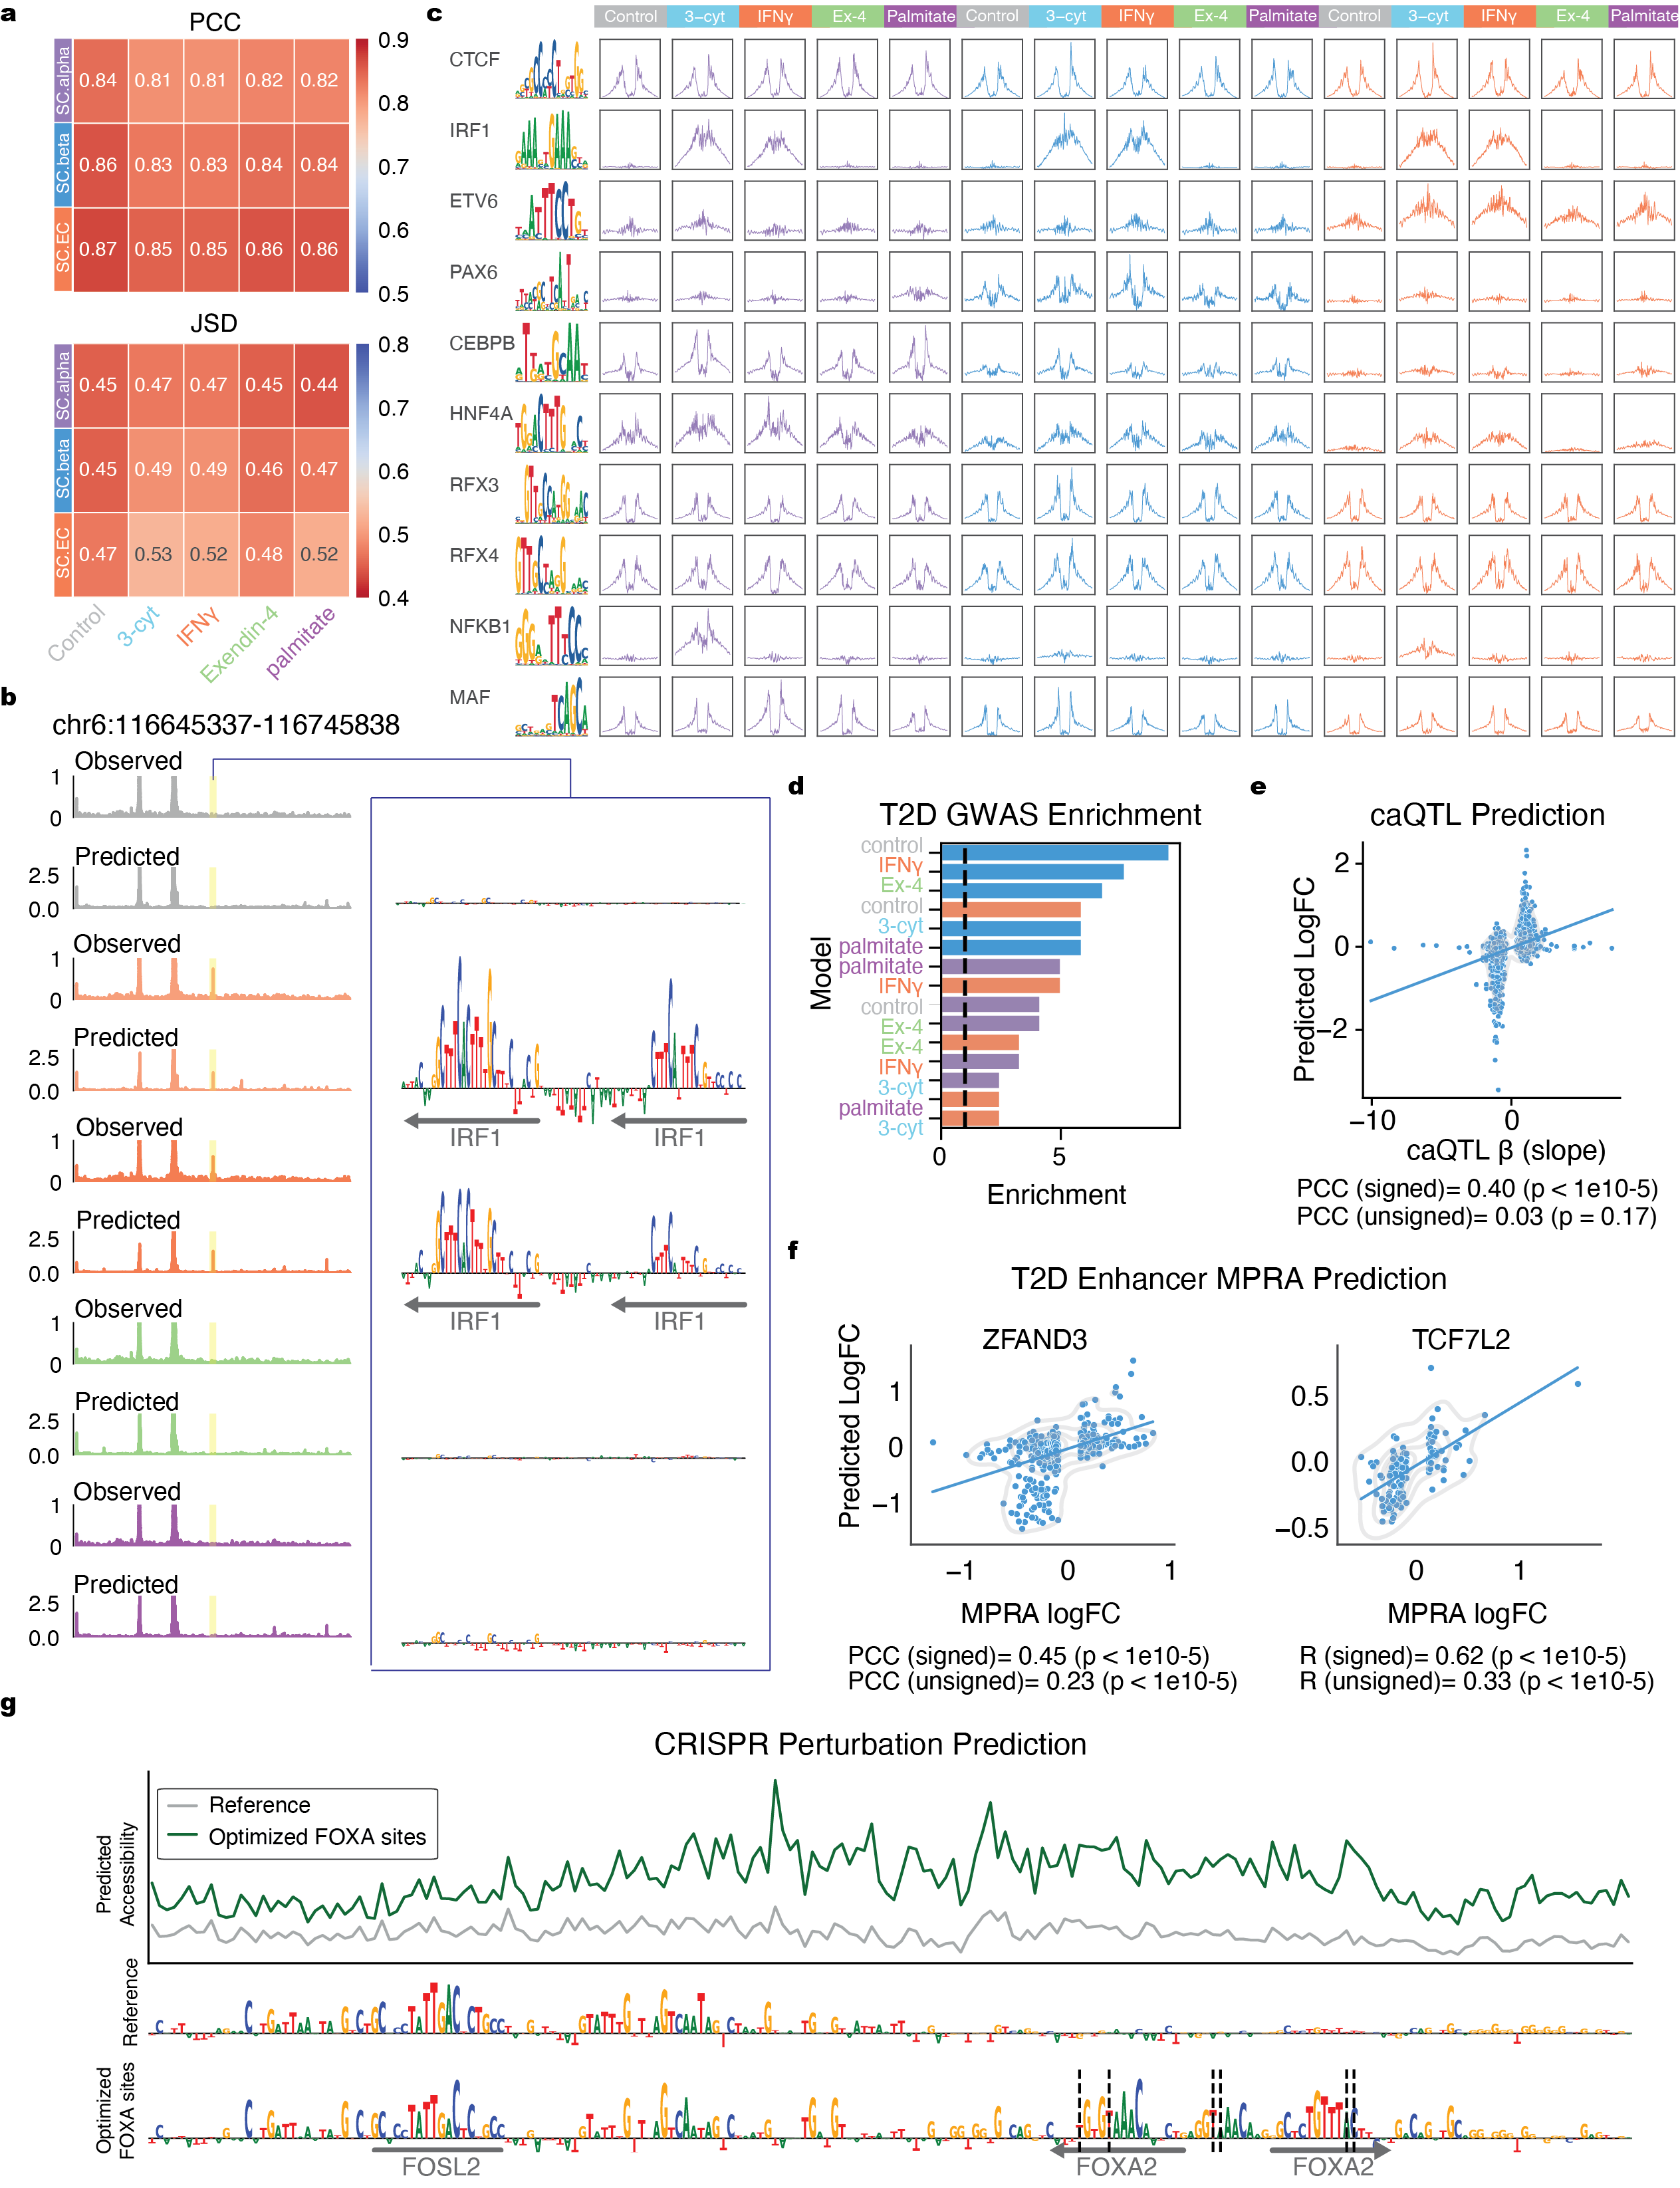
\includegraphics[width=0.9\textwidth, height=0.745\textheight]{3_figures-and-files/Fig4.png}
    \caption[Prediction of chromatin accessibility and variant effects]{\textbf{Sequence-to-function models accurately predict condition specific chromatin accessibility and regulatory variant effects}. \textbf{a}, Heatmap of Pearson’s correlation coefficients (PCCs) between observed and predicted log(Tn5 insertion counts) in peaks for ChromBPNet models trained on SC-alpha, SC-beta, and SC-EC pseudobulks across conditions. \textbf{b}, Median Jensen–Shannon divergence (JSD) in peaks between predicted and observed accessibility profiles. \textbf{c}, Representative genomic locus showing predicted and observed accessibility tracks across conditions (left) and per-base contributions for a peak that is differentially accessible in the cytokine conditions (right). \textbf{d}, Enrichment of fine-mapped T2D variants (PIP > 0.8) among the top 1\% of model-predicted variant effect scores. \textbf{e}, Correlation between predicted log fold-change and caQTL slope in human primary islets for SC-beta-control model. \textbf{f}, Correlation between predicted logFC and log fold-change from MPRA experiments in MIN6 cells at two T2D-associated loci. \textbf{g}, Predicted accessibility across a validated enhancer upstream of NKX6-1, comparing reference and FOXA2 motif–optimized sequences. Predicted contribution scores at the same locus, highlighting increased contributions at FOXA sites in the optimized sequence.}
    \label{fig:3 Figure 4}
\end{figure}

% To uncover the sequence features driving condition-specific chromatin accessibility in SC-islet organoids, we trained a series of ChromBPNet \cite{Pampari2025-lm} models on pseudobulked ATAC-seq fragments from each cell type and condition \cite{Pampari2025-lm}. All trained models showed strong performance in predicting cell type and condition-specific accessibility profiles, with Pearson correlation coefficients exceeding 0.8 for total accessibility count predictions (\textbf{Figure~\ref{fig:3 Figure 4}\textbf{a}}). Median Jensen–Shannon divergence (JSD) also confirmed the ability of models to recapitulate local accessibility profiles (\textbf{Figure~\ref{fig:3 Figure 4}\textbf{a}}). Models were capable of capturing differential accessibility across conditions (\textbf{Figure~\ref{fig:3 Figure 4}\textbf{b}}), including those observed under inflammatory stress.

% To identify learned sequence motifs that influence accessibility, we applied TF-MoDISco \cite{Shrikumar2018-sb} to base-pair contribution scores and identified short sequence motifs that drive accessibility in each context (see Methods). We then calculated an effect size for each motif and model combination by marginalizing the motif effect across a set of 100 background sequences (see Methods, \textbf{Figure~\ref{fig:3 Figure 4}\textbf{c}}). Using an ANOVA to identify motifs that were condition- and cell-type-specific, we found 7 motifs with condition specificity and 19 motifs with cell type specificity. Condition-specific motifs included the canonical IRF1 dimer \cite{Kirchhoff1998-xj}, which showed a large effect across cell types for 3-cyt and IFN$\gamma$ models, in concordance with the differential motif analysis. We also identified several cell-type-specific motifs, including PAX6 (SC-$\beta$), HNF4A (SC-$\alpha$), and ETV6 (SC-EC). Certain motifs showed both cell type and condition-specific effects, including NFKB1, which was active only in SC-$\alpha$ cells treated with 3-cyt. 

% We next tested whether the models could generalize to predict functional consequences of noncoding genetic variants in four ways. First, we looked at whether models could prioritize fine-mapped type 2 diabetes (T2D) variants from the DIAMANTE consortium \cite{Mahajan2022-hu} against a background set (see Methods). We found that model-derived variant scores were significantly enriched for high posterior inclusion probability (PIP) SNPs, particularly in SC-$\beta$ cell models (\textbf{Figure~\ref{fig:3 Figure 4}\textbf{d}}). Second, we asked whether predictions from the SC-$\beta$ control model were concordant with caQTLs in primary human islets \cite{Mummey2024-kx}. The model captured the direction of effect but mostly underestimated effect magnitude (\textbf{Figure~\ref{fig:3 Figure 4}\textbf{e}}). Third, we asked if the same SC-$\beta$ control model could predict variant effects as measured by MPRA. We used saturation mutagenesis MPRA experiments at T2D-associated enhancer loci in MIN6 cells and again evaluated the SC-$\beta$ control model \cite{Kircher2019-di} (\textbf{Figure~\ref{fig:3 Figure 4}\textbf{f}}). Predictions were strongly correlated with the experimental measurements and outperformed previous models across both loci \cite{Hudaiberdiev2023-ew}.

% Finally, we tested if the SC-$\beta$ control model could accurately recapitulate the effect of CRISPR-Cas9 edits in SC-islets \cite{Geusz2021-mr}. In this study, multiple degenerate FOXA motif sites in an enhancer for \textit{NKX6-1} were identified and optimized via CRISPR-Cas9 genome editing. These edits significantly increased enhancer activity, gene expression, and the proportion of SC-$\beta$ cells observed in the differentiation. In silico predictions with the SC-$\beta$ control model suggested a roughly twofold increase in chromatin accessibility at the enhancer that contained these optimized edits compared to the reference sequence, along with a predicted increase in FOXA2 binding at two of the four sites (\textbf{Figure~\ref{fig:3 Figure 4}\textbf{g}}). Overall, these results suggest that sequence-to-function models trained on snATAC-seq data from SC-islets can be used to identify candidate functional variants and propose mechanisms for their action.

\subsection{Predicting DNA methylation levels via sequence models}

\begin{figure}[p]
    \centering
    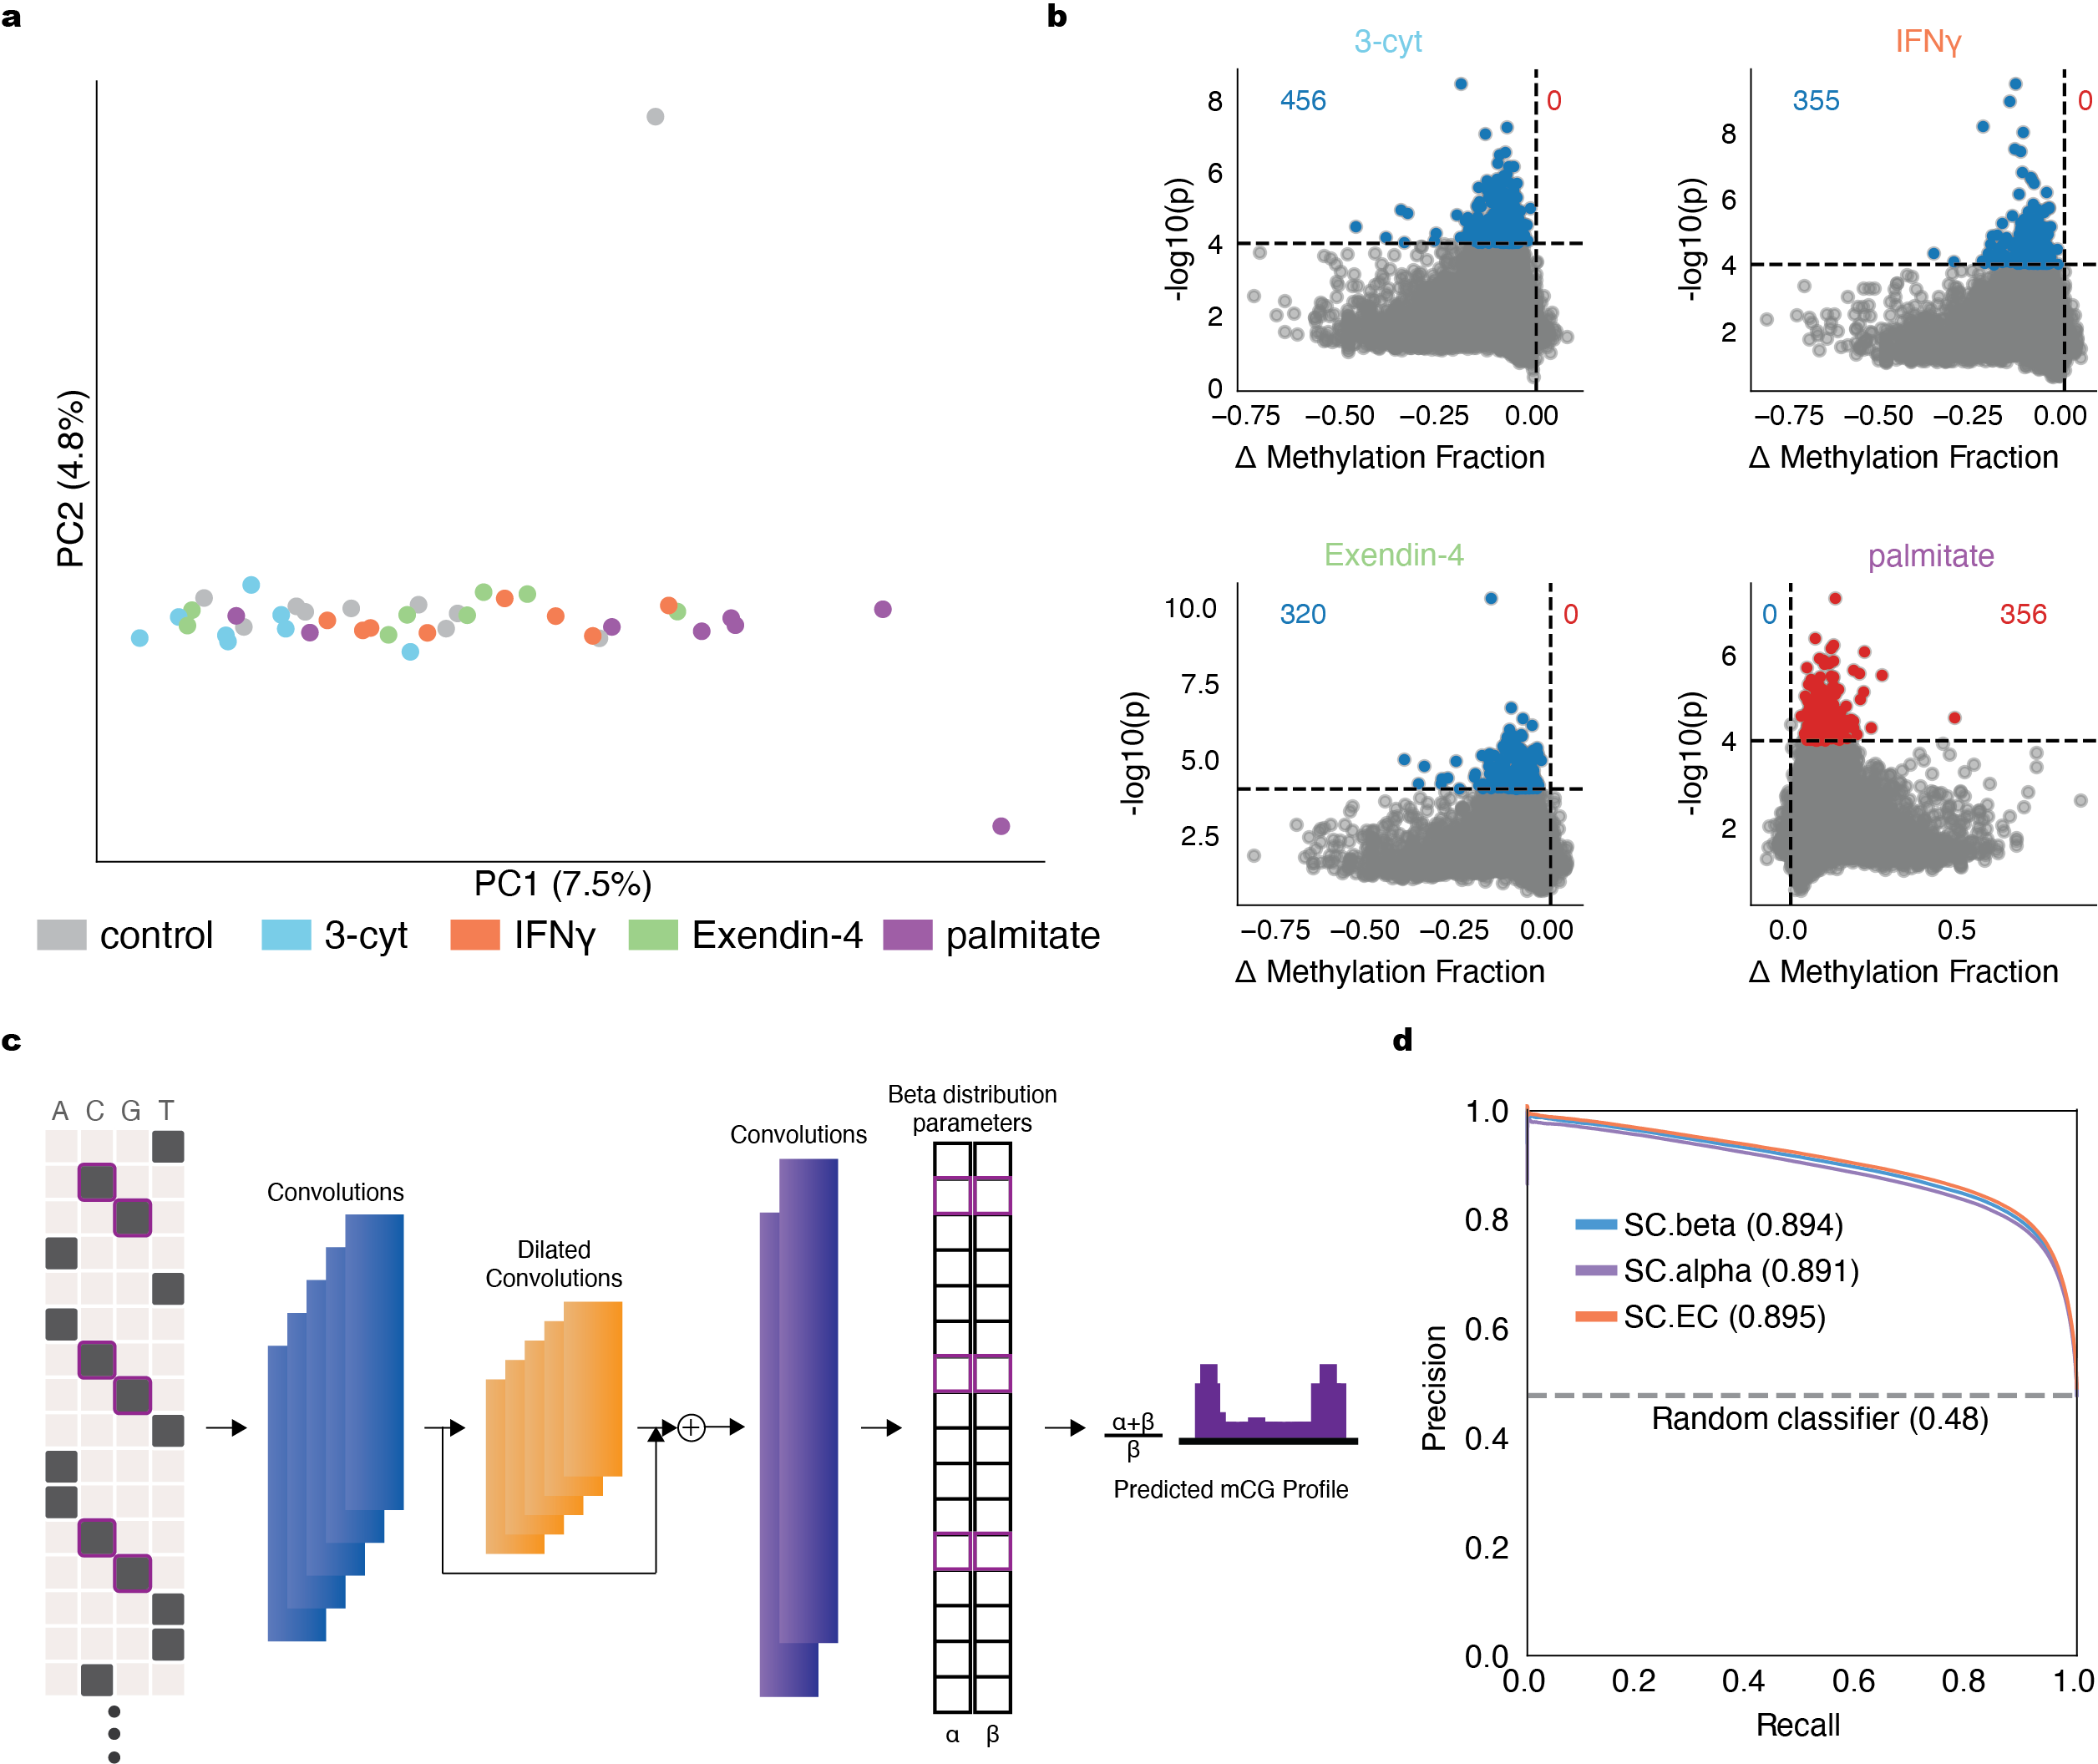
\includegraphics[width=0.9\textwidth, height=0.745\textheight]{3_figures-and-files/Fig5.png}
    \caption[CpG methylation prediction across cell types]{\textbf{Sequence-to-function models accurately classify CpG methylation across cell types}. \textbf{a}, Principal component analysis of pseudobulked DNA methylation profiles from SC-beta cells across all treatment conditions and time points. \textbf{b}, Volcano plots showing differential DNA methylation in SC-beta cells across treatments (relative to control). From top left to bottom right: 3-cyt, IFNg, Ex-4\_HG, and palmitate. Positive $\Delta$ indicates increased methylation; negative indicates decreased. Colored points indicate sites with nominal p-value < 0.0001, red-increased, blue-decreased. \textbf{f}, Schematic of deep learning model for predicting methylation profiles from sequence (CpGNet). CpGNet predicts parameters of a beta distribution ($\alpha$, $\beta$) for each CpG in a 2,114 bp window. The parameters can be converted to a point estimate of the methylation fraction using the indicated formula. \textbf{g}, Precision–recall curves showing classification performance of methylation models across cell types. Area under the PR curve (auPRC) is reported for each model in parentheses. The gray dashed line represents the performance of a random classifier.}
    \label{fig:3 Figure 5}
\end{figure}

% We next examined how DNA methylation changes in SC-$\beta$ cells in response to environmental stimuli. While strong cell-type–specific differences in methylation at CpGs were observed (\textbf{Figure~\ref{fig:3 Figure 1}\textbf{b}}), condition-specific effects within SC-$\beta$ cells were comparatively modest (\textbf{Figure~\ref{fig:3 Figure 5}\textbf{a}}). Differential methylation analysis identified fewer than 10 significantly altered regions at a canonical 5\% FDR. Applying a relaxed nominal $p$-value cutoff ($p < 0.0001$), we were able to observe global trends in DNA methylation changes. Specifically, treatment with 3-cyt, IFN$\gamma$, and Exendin-4 was associated with a global decrease in methylation, whereas palmitate exposure induced modest methylation gains across many loci (\textbf{Figure~\ref{fig:3 Figure 5}\textbf{b}}). The subtlety of these observed patterns may reflect a lack of a strong effect of these stimuli on CpG methylation, but it remains possible that the timeframe we used is insufficient to capture more extensive DNA methylation changes.

% To better understand the sequence determinants of methylation, we aimed to develop deep learning models that predict DNA methylation profiles from sequence. Unlike prior models of this type, which often predict binary methylation states at individual CpGs or average methylation across regions \cite{Zeng2017-kb}, our approach aims to improve resolution on both fronts. Specifically, we devised a modeling framework in which we predict the parameters of a beta distribution for each CpG site within a 2,114 bp sequence window. This approach provides a measure of uncertainty in the prediction at a given site, while also allowing for point estimates of methylation fractions for performance comparisons (\textbf{Figure~\ref{fig:3 Figure 5}\textbf{c}}). While quantitative prediction performance was modest, classification accuracy was strong across SC-$\alpha$, SC-$\beta$, and SC-EC models (\textbf{Figure~\ref{fig:3 Figure 5}\textbf{d}}). These results suggest that cell-type–specific methylation patterns are at least partially encoded in the underlying DNA sequence.

